\section*{Modulebeschrijving}
\begin{tabularx}{\textwidth}{|>{\columncolor{lichtGrijs}} p{.26\textwidth}|X|}
	\hline
	\textbf{Modulenaam:} & \modulenaam\\
	\hline
	\textbf{Modulecode: }& \modulecode\\
	\hline
	\textbf{Aantal studiepunten \newline en studiebelastinguren:} & Deze module levert \stdPunten studiepunten op, hetgeen overeenkomt met 84 uur.
	\begin{itemize}
		\item 8 $\times$ 120 minuten hoorcollege
		\item 8 $\times$ 120 minuten practicum
		\item 12 $\times$ 120 minuten zelfstudie
	\end{itemize} \\
	\hline
	\textbf{Toetsing:} & Practicumopdrachten \\
	\hline
	\textbf{Werkvorm:} & Hoorcollege en practicum \\
	\hline
	\textbf{Vereiste voorkennis:}&Alle modules wiskunde en programmeren uit het eerste jaar en de eerste helft van het tweede jaar.\\
	\hline
	\textbf{Leermiddelen:}  &
		\begin{itemize}
			\item Boek: Types and Programming Languages, auteur: Benjamin Pierce
			\item Boek: Friendly F\# (Fun with game programming Book 1), auteurs: Giuseppe Maggiore, Giulia Costantini
			\item Text editors: Emacs, Notepad++, Visual Studio, Xamarin Studio, etc.
		\end{itemize} \\
	\hline
	\textbf{Draagt bij aan \newline competenties:} &
	\begin{center}
		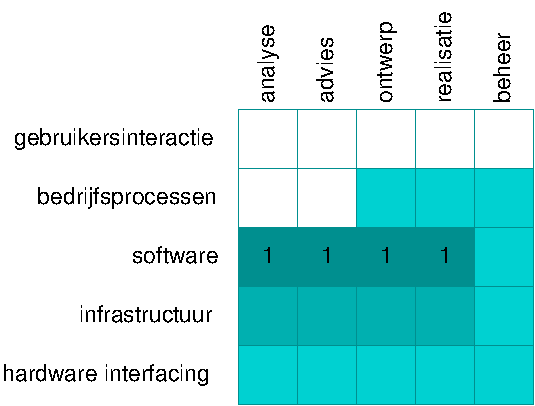
\includegraphics[width=7cm]{img/comptabel.pdf}
	\end{center}\\
	\hline
	\textbf{Leerdoelen:}&
	\begin{itemize}
		\item Het kunnen adviseren over en analyseren, ontwerpen en realiseren van een computerprogramma op niveau 1 (leerdoel A).
		\item Het kunnen ontwerpen, schrijven, compileren en uitvoeren van een correct werkend ML programma (leerdoel O).
		\item Het in correct Nederlands en met gebruikmaking van het juiste jargon kunnen communiceren over de programmeertaal (leerdoel C).
	\end{itemize} \\
	\hline
\end{tabularx}
\newpage

\begin{tabularx}{\textwidth}{|>{\columncolor{lichtGrijs}} p{.26\textwidth}|X|}
	\hline
	\textbf{Inhoud:}&
	\begin{itemize}
		\item Programmeerparadigma's;
		\item Waarden en \texttt{let};
		\item Functies en recursieve functies
		\item Data structuren;
		\item Recursieve data structuren: lijsten, bomen;
		\item Hogere orde functies: \texttt{map}, \texttt{filter};
		\item Abstractie door records van functies;
		\item Staart recursie, accumulatoren, \textit{continuation passing style}.
	\end{itemize}\\
	\hline
	\textbf{Modulebeheerder:} & \author\\
	\hline
	\textbf{Datum:} & \today \\
	\hline
\end{tabularx}
\newpage